

\tikzset{every picture/.style={line width=0.75pt}} %set default line width to 0.75pt        

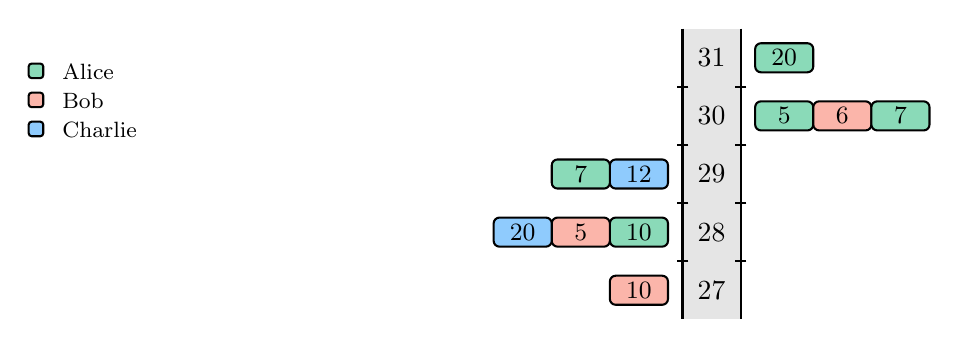
\begin{tikzpicture}[x=0.75pt,y=0.75pt,yscale=-0.7,xscale=0.7]
%%uncomment if require: \path (0,300); %set diagram left start at 0, and has height of 300

%Shape: Rectangle [id:dp8091118426371228] 
\draw  [draw opacity=0][fill={rgb, 255:red, 0; green, 0; blue, 0 }  ,fill opacity=0.1 ] (480,70) -- (520,70) -- (520,270) -- (480,270) -- cycle ;
%Rounded Rect [id:dp03190620142202172] 
\draw  [fill={rgb, 255:red, 138; green, 218; blue, 184 }  ,fill opacity=1 ][line width=0.75]  (530,124) .. controls (530,121.79) and (531.79,120) .. (534,120) -- (566,120) .. controls (568.21,120) and (570,121.79) .. (570,124) -- (570,136) .. controls (570,138.21) and (568.21,140) .. (566,140) -- (534,140) .. controls (531.79,140) and (530,138.21) .. (530,136) -- cycle ;
%Straight Lines [id:da22911621952375028] 
\draw    (480,70) -- (480,270) (484,110) -- (476,110)(484,150) -- (476,150)(484,190) -- (476,190)(484,230) -- (476,230) ;
%Straight Lines [id:da555722728776089] 
\draw    (520,70) -- (520,270) (524,110) -- (516,110)(524,150) -- (516,150)(524,190) -- (516,190)(524,230) -- (516,230) ;
%Rounded Rect [id:dp04327399535927834] 
\draw  [fill={rgb, 255:red, 251; green, 181; blue, 170 }  ,fill opacity=1 ][line width=0.75]  (570,124) .. controls (570,121.79) and (571.79,120) .. (574,120) -- (606,120) .. controls (608.21,120) and (610,121.79) .. (610,124) -- (610,136) .. controls (610,138.21) and (608.21,140) .. (606,140) -- (574,140) .. controls (571.79,140) and (570,138.21) .. (570,136) -- cycle ;
%Rounded Rect [id:dp8469096370209764] 
\draw  [fill={rgb, 255:red, 138; green, 218; blue, 184 }  ,fill opacity=1 ][line width=0.75]  (610,124) .. controls (610,121.79) and (611.79,120) .. (614,120) -- (646,120) .. controls (648.21,120) and (650,121.79) .. (650,124) -- (650,136) .. controls (650,138.21) and (648.21,140) .. (646,140) -- (614,140) .. controls (611.79,140) and (610,138.21) .. (610,136) -- cycle ;
%Rounded Rect [id:dp9977116236845125] 
\draw  [fill={rgb, 255:red, 138; green, 218; blue, 184 }  ,fill opacity=1 ][line width=0.75]  (530,84) .. controls (530,81.79) and (531.79,80) .. (534,80) -- (566,80) .. controls (568.21,80) and (570,81.79) .. (570,84) -- (570,96) .. controls (570,98.21) and (568.21,100) .. (566,100) -- (534,100) .. controls (531.79,100) and (530,98.21) .. (530,96) -- cycle ;
%Rounded Rect [id:dp40669282343922186] 
\draw  [fill={rgb, 255:red, 138; green, 218; blue, 184 }  ,fill opacity=1 ][line width=0.75]  (430,204) .. controls (430,201.79) and (431.79,200) .. (434,200) -- (466,200) .. controls (468.21,200) and (470,201.79) .. (470,204) -- (470,216) .. controls (470,218.21) and (468.21,220) .. (466,220) -- (434,220) .. controls (431.79,220) and (430,218.21) .. (430,216) -- cycle ;
%Rounded Rect [id:dp9142536483866215] 
\draw  [fill={rgb, 255:red, 143; green, 203; blue, 253 }  ,fill opacity=1 ][line width=0.75]  (430,164) .. controls (430,161.79) and (431.79,160) .. (434,160) -- (466,160) .. controls (468.21,160) and (470,161.79) .. (470,164) -- (470,176) .. controls (470,178.21) and (468.21,180) .. (466,180) -- (434,180) .. controls (431.79,180) and (430,178.21) .. (430,176) -- cycle ;
%Rounded Rect [id:dp9348427490425627] 
\draw  [fill={rgb, 255:red, 138; green, 218; blue, 184 }  ,fill opacity=1 ][line width=0.75]  (390,164) .. controls (390,161.79) and (391.79,160) .. (394,160) -- (426,160) .. controls (428.21,160) and (430,161.79) .. (430,164) -- (430,176) .. controls (430,178.21) and (428.21,180) .. (426,180) -- (394,180) .. controls (391.79,180) and (390,178.21) .. (390,176) -- cycle ;
%Rounded Rect [id:dp2667271005175228] 
\draw  [fill={rgb, 255:red, 251; green, 181; blue, 170 }  ,fill opacity=1 ][line width=0.75]  (390,204) .. controls (390,201.79) and (391.79,200) .. (394,200) -- (426,200) .. controls (428.21,200) and (430,201.79) .. (430,204) -- (430,216) .. controls (430,218.21) and (428.21,220) .. (426,220) -- (394,220) .. controls (391.79,220) and (390,218.21) .. (390,216) -- cycle ;
%Rounded Rect [id:dp5911982178413685] 
\draw  [fill={rgb, 255:red, 143; green, 203; blue, 253 }  ,fill opacity=1 ][line width=0.75]  (350,204) .. controls (350,201.79) and (351.79,200) .. (354,200) -- (386,200) .. controls (388.21,200) and (390,201.79) .. (390,204) -- (390,216) .. controls (390,218.21) and (388.21,220) .. (386,220) -- (354,220) .. controls (351.79,220) and (350,218.21) .. (350,216) -- cycle ;
%Rounded Rect [id:dp9977666228162302] 
\draw  [fill={rgb, 255:red, 251; green, 181; blue, 170 }  ,fill opacity=1 ][line width=0.75]  (430,244) .. controls (430,241.79) and (431.79,240) .. (434,240) -- (466,240) .. controls (468.21,240) and (470,241.79) .. (470,244) -- (470,256) .. controls (470,258.21) and (468.21,260) .. (466,260) -- (434,260) .. controls (431.79,260) and (430,258.21) .. (430,256) -- cycle ;
%Rounded Rect [id:dp0318183239720361] 
\draw  [fill={rgb, 255:red, 138; green, 218; blue, 184 }  ,fill opacity=1 ][line width=0.75]  (30,96) .. controls (30,94.9) and (30.9,94) .. (32,94) -- (38,94) .. controls (39.1,94) and (40,94.9) .. (40,96) -- (40,102) .. controls (40,103.1) and (39.1,104) .. (38,104) -- (32,104) .. controls (30.9,104) and (30,103.1) .. (30,102) -- cycle ;
%Rounded Rect [id:dp16680821822273184] 
\draw  [fill={rgb, 255:red, 143; green, 203; blue, 253 }  ,fill opacity=1 ][line width=0.75]  (30,136) .. controls (30,134.9) and (30.9,134) .. (32,134) -- (38,134) .. controls (39.1,134) and (40,134.9) .. (40,136) -- (40,142) .. controls (40,143.1) and (39.1,144) .. (38,144) -- (32,144) .. controls (30.9,144) and (30,143.1) .. (30,142) -- cycle ;
%Rounded Rect [id:dp4425250472328628] 
\draw  [fill={rgb, 255:red, 251; green, 181; blue, 170 }  ,fill opacity=1 ][line width=0.75]  (30,116) .. controls (30,114.9) and (30.9,114) .. (32,114) -- (38,114) .. controls (39.1,114) and (40,114.9) .. (40,116) -- (40,122) .. controls (40,123.1) and (39.1,124) .. (38,124) -- (32,124) .. controls (30.9,124) and (30,123.1) .. (30,122) -- cycle ;

% Text Node
\draw (500,90) node    {$31$};
% Text Node
\draw (500,129.5) node    {$30$};
% Text Node
\draw (550,130) node  [font=\small]  {${\textstyle 5}$};
% Text Node
\draw (500,170) node    {$29$};
% Text Node
\draw (500,210) node    {$28$};
% Text Node
\draw (500,250) node    {$27$};
% Text Node
\draw (590,130) node  [font=\small]  {$6$};
% Text Node
\draw (630,130) node  [font=\small]  {$7$};
% Text Node
\draw (550,90) node  [font=\small]  {$20$};
% Text Node
\draw (450,210) node  [font=\small]  {$10$};
% Text Node
\draw (450,170) node  [font=\small]  {$12$};
% Text Node
\draw (410,170) node  [font=\small]  {$7$};
% Text Node
\draw (410,210) node  [font=\small]  {${\textstyle 5}$};
% Text Node
\draw (370,210) node  [font=\small]  {$20$};
% Text Node
\draw (450,250) node  [font=\small]  {$10$};
% Text Node
\draw (51,92) node [anchor=north west][inner sep=0.75pt]  [font=\footnotesize] [align=left] {Alice};
% Text Node
\draw (51,112) node [anchor=north west][inner sep=0.75pt]  [font=\footnotesize] [align=left] {Bob};
% Text Node
\draw (51,132) node [anchor=north west][inner sep=0.75pt]  [font=\footnotesize] [align=left] {Charlie};


\end{tikzpicture}
